\section{Models}
\label{sec:models}

\textbf{What is predicted.} One model per case maps the 12 inputs (vdd, temp, w, vd, vs, vg, vb and the five process parameters) to the four terminal currents $(I_d,I_g,I_s,I_b)$. The models do not predict the raw currents. Because currents span many decades, the targets are natural logarithms: the positive channel conductances $G_d=(I_d+H)/\Delta V$ and $G_s=-(I_s+H)/\Delta V$, where $\Delta V$ is the voltage difference across the channel and $H=(I_g+I_b)/2$, plus $\ln|I_g|$ and $\ln|I_b|$. Conductances and $|I_g|$ are divided by $(W-\SI{10}{\nano\meter})/\SI{100}{\nano\meter}$ before taking the logarithm. The signs and the drain/source order are restored afterwards, so each model returns the four signed currents. Inputs are pre-processed with the same transformations for all four model types: PMOS polarity is flipped, drain and source are ordered by potential, and smooth functions of temperature, width and process values (for example $1/\mathrm{toxe}$ and $\ln\mathrm{ndep}$) are added. All fitted scaling uses training rows only.

\textbf{Baselines and the ON gate-edge residual.} For the OFF cases the gate-current baseline is the fixed BSIM gate-to-diffusion edge expression with the parameters of the supplied model card, and the model learns its logarithmic residual. The body baseline is $5\times10^{-15}\,\mathrm{A}\times[2-e^{-V_{low}/V_T}-e^{-V_{high}/V_T}]$. This body scale and the junction-coordinate warp are numerical conditioning choices, not exact BSIM body equations. For the ON cases a second local RBF learns $\ln\!\big(|I_g|/|I_{edge,source}+I_{edge,drain}|\big)$; half of its gate-current change is compensated in each of the drain and source predictions, so the learned channel difference and the raw KCL residual are preserved. At zero edge voltage this ON gate baseline omits the tiny gate-to-body tunnelling current; its raw-current error remains visible in the boundary diagnostics. The coefficients and the current reconstruction are in \texttt{code/lusr/physics\_surrogate.py} and \texttt{code/lusr/smooth\_models.py}. No SPICE call is made at inference.

\textbf{Four model types.} Table~\ref{tab:hyper} lists the families and their main hyperparameters. The last family is a local radial-basis-function (RBF) interpolator (scipy \texttt{RBFInterpolator}). It is a kernel regression model fitted to transistor data only, with no SPICE call at prediction time.

\begin{table}[H]
\centering\small
\caption{Model families and main hyperparameters.}
\label{tab:hyper}
\begin{tabular}{lp{11cm}}
\toprule
Family & Main hyperparameters \\
\midrule
Random forest & 128 trees, all features, unlimited depth, minimum leaf size 2, seed 20261024 \\
Extra trees & same settings as the random forest \\
Hist. gradient boosting & one regressor per target, 400 iterations, learning rate 0.08, 63 leaves, minimum leaf 15, L2 penalty 0.01 \\
Local quintic RBF & quintic kernel, degree-2 polynomial term, smoothing $10^{-12}$, nearest 512 training points (NMOS OFF) or 256 (other cases). The ON models add a second RBF (256 neighbours) for the gate-edge tunnelling current. \\
\bottomrule
\end{tabular}
\end{table}

\textbf{Comparison.} Table~\ref{tab:val} gives the validation results. The RBF has the lowest median and 95th-percentile error in all four cases, by one to three orders of magnitude for the median. For the two OFF cases gradient boosting has a higher linear $R^2$ than the RBF on validation (0.949 against 0.914 for NMOS OFF and 0.982 against 0.959 for PMOS OFF). That $R^2$ is dominated by the few largest currents and does not measure percentage accuracy, so it was not used for the choice. The test-set $R^2$ of the chosen models is discussed below.

\begin{table}[H]
\centering
\small
\caption{Model comparison on the validation split (15,000 rows per case, pooled over the four terminal currents). The last column is the single-FET power/VDD error on the separate 512-row rail-boundary set (Section~\ref{sec:models}). The selected model is in bold.}
\label{tab:val}
\resizebox{\ifdim\width>\linewidth\linewidth\else\width\fi}{!}{%
\begin{tabular}{llrrrr}
\toprule
Case & Model & $R^2$ & Median err. (\%) & p95 err. (\%) & Rail-set power MAPE (\%) \\
\midrule
nmos\_on & Random forest & 0.9548 & 10.98 & 56.5 & 27.1 \\
 & Extra trees & 0.9644 & 9.045 & 46.4 & 25.4 \\
 & Hist. gradient boosting & 0.9950 & 2.756 & 19.8 & 4.53 \\
 & \textbf{Local quintic RBF} & 1.0000 & 0.06838 & 1.38 & 0.169 \\
nmos\_off & Random forest & 0.9046 & 2.111 & 42 & 103 \\
 & Extra trees & 0.8909 & 1.328 & 33.6 & 83 \\
 & Hist. gradient boosting & 0.9487 & 1.436 & 23.6 & 73.2 \\
 & \textbf{Local quintic RBF} & 0.9142 & 0.003451 & 5.18 & 1.23 \\
pmos\_on & Random forest & 0.9665 & 9.822 & 50.8 & 25.9 \\
 & Extra trees & 0.9744 & 8.338 & 40.7 & 24.7 \\
 & Hist. gradient boosting & 0.9969 & 2.148 & 18.2 & 7.72 \\
 & \textbf{Local quintic RBF} & 1.0000 & 0.03614 & 1.08 & 0.316 \\
pmos\_off & Random forest & 0.9469 & 1.971 & 36.9 & 56 \\
 & Extra trees & 0.9385 & 1.324 & 29.7 & 40.3 \\
 & Hist. gradient boosting & 0.9816 & 1.347 & 19.9 & 25.7 \\
 & \textbf{Local quintic RBF} & 0.9585 & 0.01618 & 5.2 & 1.2 \\
\bottomrule
\end{tabular}%
}
\end{table}


\textbf{Final choice per case.}
\begin{itemize}
\item \emph{NMOS ON and PMOS ON: local quintic RBF.} Validation median error 0.068\% and 0.036\%, against 2.8\% and 2.2\% for the best tree-type model (boosting). $R^2>0.999998$ and the lowest rail-set error.
\item \emph{NMOS OFF and PMOS OFF: local quintic RBF (512 and 256 neighbours).} Validation median error 0.0035\% and 0.016\%, against 1.4\% (boosting) for both. The 95th-percentile error is about 5.2\% against about 20--24\% for boosting. The rail-set power error is 1.2\% against 73\% (NMOS OFF) and 26\% (PMOS OFF) for boosting.
\end{itemize}
The OFF models also use a physics baseline for the gate and body currents (below).

\textbf{Disclosures about the selection.}
\begin{enumerate}
\item \emph{Physics-informed baselines.} The RBF models predict the logarithmic residual relative to fixed analytic baselines taken from the BSIM4 equations and the constants of the 32nm\_MGK model card: the gate-to-diffusion edge tunnelling current (for OFF gate current, and for the ON gate-edge residual), and a body-current baseline $5\times10^{-15}\,\mathrm{A}\times[2-e^{-V_{low}/V_T}-e^{-V_{high}/V_T}]$, which is a conditioning choice and not an exact BSIM expression. The tree models do not receive these baselines, so the comparison is not like for like. It also means the final models are physics-informed ML and would need new baselines for another technology. Only transistor data is used for fitting.
\item \emph{Extra rail-boundary set.} Selection used a predeclared score: the error of the single-FET power divided by $V_{DD}$ on a separate set of 512 transistor samples per case (seed 2026102407) at or near the supply rails, where gate terminals sit in practice. This set is not part of the training data and does not come from gate or circuit corners; its last column in Table~\ref{tab:val} is shown for all families. Validation rows were used to break ties. The selection script (\texttt{code/scripts/13\_prepare\_revision\_selection.py}) stops with an error if any tree beats the RBF on this score. The same choice follows from plain validation median and p95 error (Table~\ref{tab:val}).
\item \emph{Indirect tuning.} The RBF design came from exploratory experiments after an earlier 10,000-row run gave weaker circuit accuracy. The rail-boundary set and the ON gate-edge residual were motivated by that shortfall. No gate or circuit labels were used for fitting or selection, and the final gate and circuit corners are new draws, but the development history means the gate and circuit results are not completely blind.
\item \emph{Test set.} The test rows were used once, after the models were frozen.
\end{enumerate}

\textbf{Test results.} Table~\ref{tab:pooled} gives the pooled test results and Table~\ref{tab:term} the per-terminal results. Figure~\ref{fig:parity4} shows predicted against SPICE currents for each case.

\begin{table}[H]
\centering
\small
\caption{Test-set metrics of the chosen models, pooled over the four terminals. The last column is the accuracy of the dissipated power divided by VDD for a single FET.}
\label{tab:pooled}
\resizebox{\ifdim\width>\linewidth\linewidth\else\width\fi}{!}{%
\begin{tabular}{lrrrrr}
\toprule
Case & $R^2$ (linear) & Median (\%) & p95 (\%) & Mean acc. (\%) & Power/VDD mean acc. (\%) \\
\midrule
nmos\_on & 1.0000 & 0.0675 & 1.31 & 99.69 & 99.76 \\
nmos\_off & 0.8274 & 0.00376 & 4.87 & 95.98 & 99.91 \\
pmos\_on & 1.0000 & 0.037 & 1.08 & 99.72 & 99.83 \\
pmos\_off & 0.9693 & 0.0137 & 4.77 & 83.42 & 99.87 \\
\bottomrule
\end{tabular}%
}
\end{table}


\textbf{Linear $R^2$ for the OFF cases.} The pooled linear $R^2$ is 0.827 (NMOS OFF) and 0.969 (PMOS OFF), below the 0.99 level. It is not a sign of poor percentage accuracy. In the OFF cases the pooled values include the body current $I_b$ (about $10^{-14}$\,A), and for NMOS OFF its own linear $R^2$ is 0.31 and for PMOS OFF 0.88, which pulls the average down. The drain and source currents have linear $R^2$ above 0.99997 and $R^2$ on $\log|I|$ of 0.994 to 0.998. Subthreshold current has a large dynamic range, so linear $R^2$ is set by the few largest currents. The ON cases have linear $R^2$ above 0.99999 and log $R^2$ above 0.9998.

\textbf{Terminals that are weak.} OFF-state $I_d$ and $I_s$ have median error about 0.02\% but a 95th percentile of 2.6 to 2.9\%. The OFF body current $I_b$ is an almost noise-like junction current of about $10^{-14}$\,A with a 95th-percentile error of about 26\%. It has no visible effect on gate totals. The mean accuracy of 42\% for PMOS OFF $I_s$ is caused by a few near-zero reference values, so median and p95 should be used for that terminal. The OFF gate currents are essentially exact.

\begin{table}[H]
\centering
\small
\caption{Test-set metrics per terminal (15,000 held-out rows per case).}
\label{tab:term}
\resizebox{\ifdim\width>\linewidth\linewidth\else\width\fi}{!}{%
\begin{tabular}{llrrrr}
\toprule
Case & Terminal & Median (\%) & p95 (\%) & $R^2$ on $\log|I|$ & $R^2$ linear \\
\midrule
nmos\_on & Id & 0.0703 & 1.09 & 0.99999 & 1.00000 \\
 & Ig & 0.0593 & 2.22 & 0.99998 & 1.00000 \\
 & Is & 0.0703 & 1.09 & 0.99992 & 1.00000 \\
 & Ib & 0.072 & 0.963 & 1.00000 & 1.00000 \\
nmos\_off & Id & 0.0216 & 2.58 & 0.99567 & 0.99998 \\
 & Ig & 2.77e-08 & 5.02e-07 & 1.00000 & 1.00000 \\
 & Is & 0.0205 & 2.72 & 0.99607 & 0.99998 \\
 & Ib & 0.0843 & 26.4 & 0.38075 & 0.30954 \\
pmos\_on & Id & 0.0303 & 0.816 & 0.99999 & 1.00000 \\
 & Ig & 0.0571 & 3.39 & 0.99989 & 1.00000 \\
 & Is & 0.0302 & 0.815 & 0.99999 & 1.00000 \\
 & Ib & 0.0337 & 0.704 & 1.00000 & 1.00000 \\
pmos\_off & Id & 0.0202 & 2.83 & 0.99765 & 0.99998 \\
 & Ig & 1.27e-05 & 0.000454 & 1.00000 & 1.00000 \\
 & Is & 0.0207 & 2.92 & 0.99372 & 0.99998 \\
 & Ib & 0.154 & 25.7 & 0.58589 & 0.87732 \\
\bottomrule
\end{tabular}%
}
\end{table}


\begin{figure}[H]
\centering
\begin{subfigure}[t]{0.49\linewidth}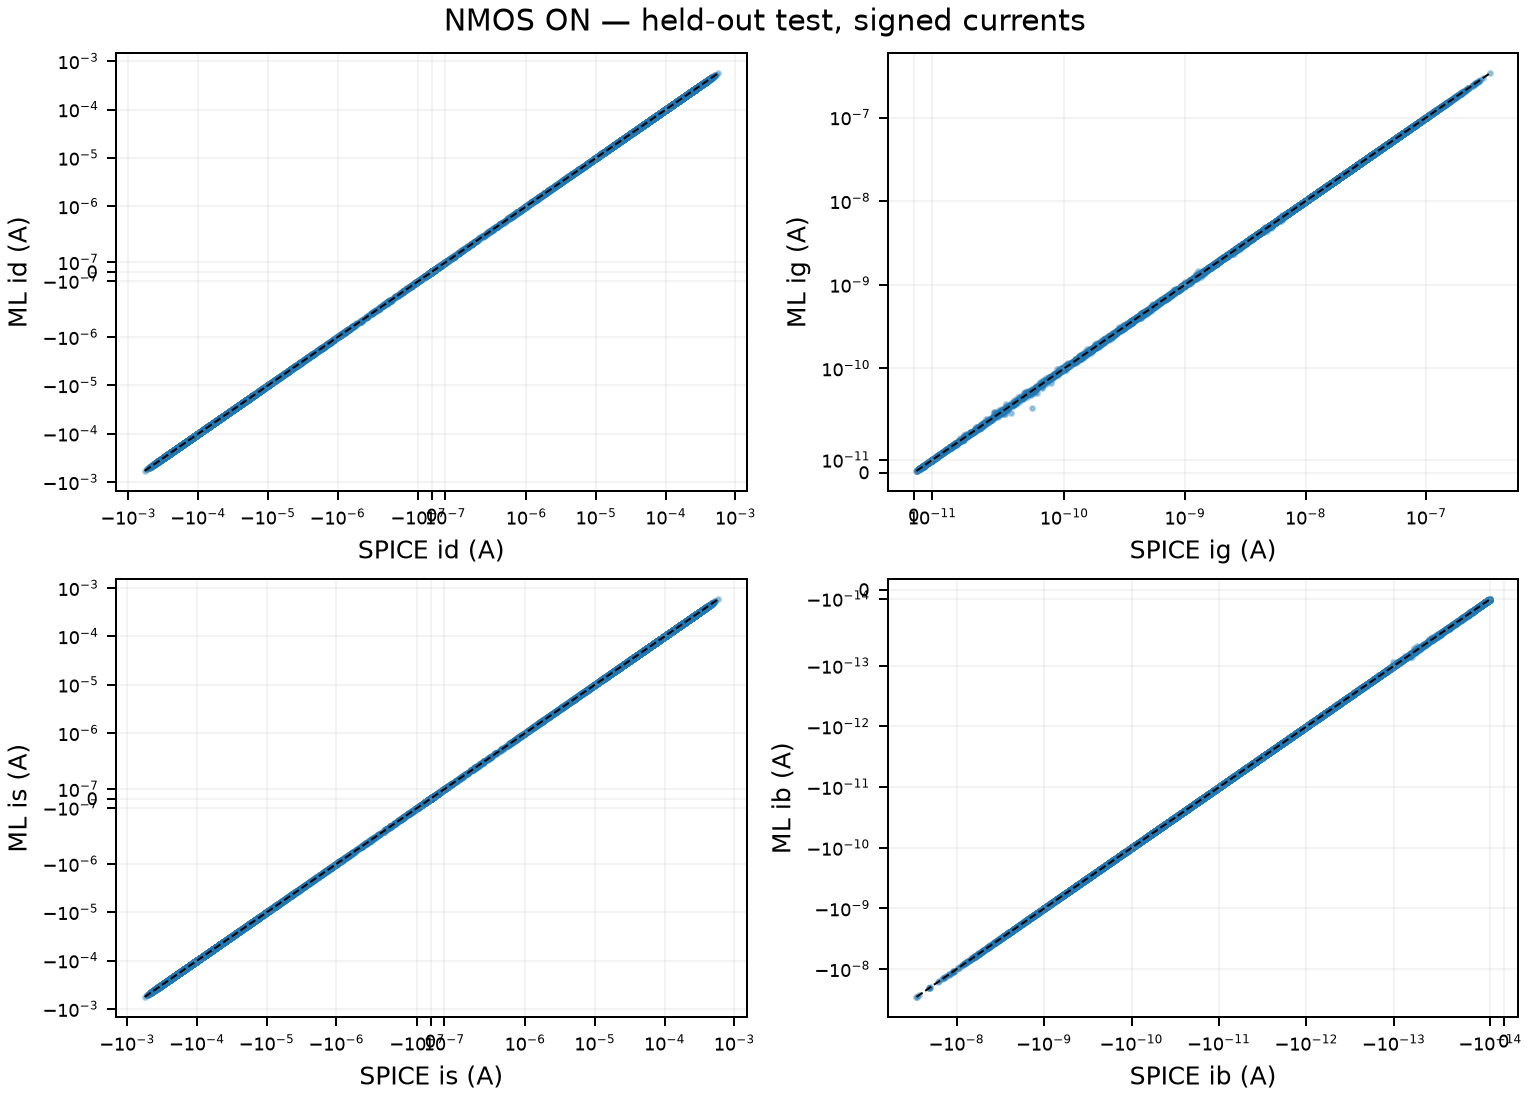
\includegraphics[width=\linewidth]{figures/nmos_on_parity.png}\caption{NMOS ON}\end{subfigure}
\begin{subfigure}[t]{0.49\linewidth}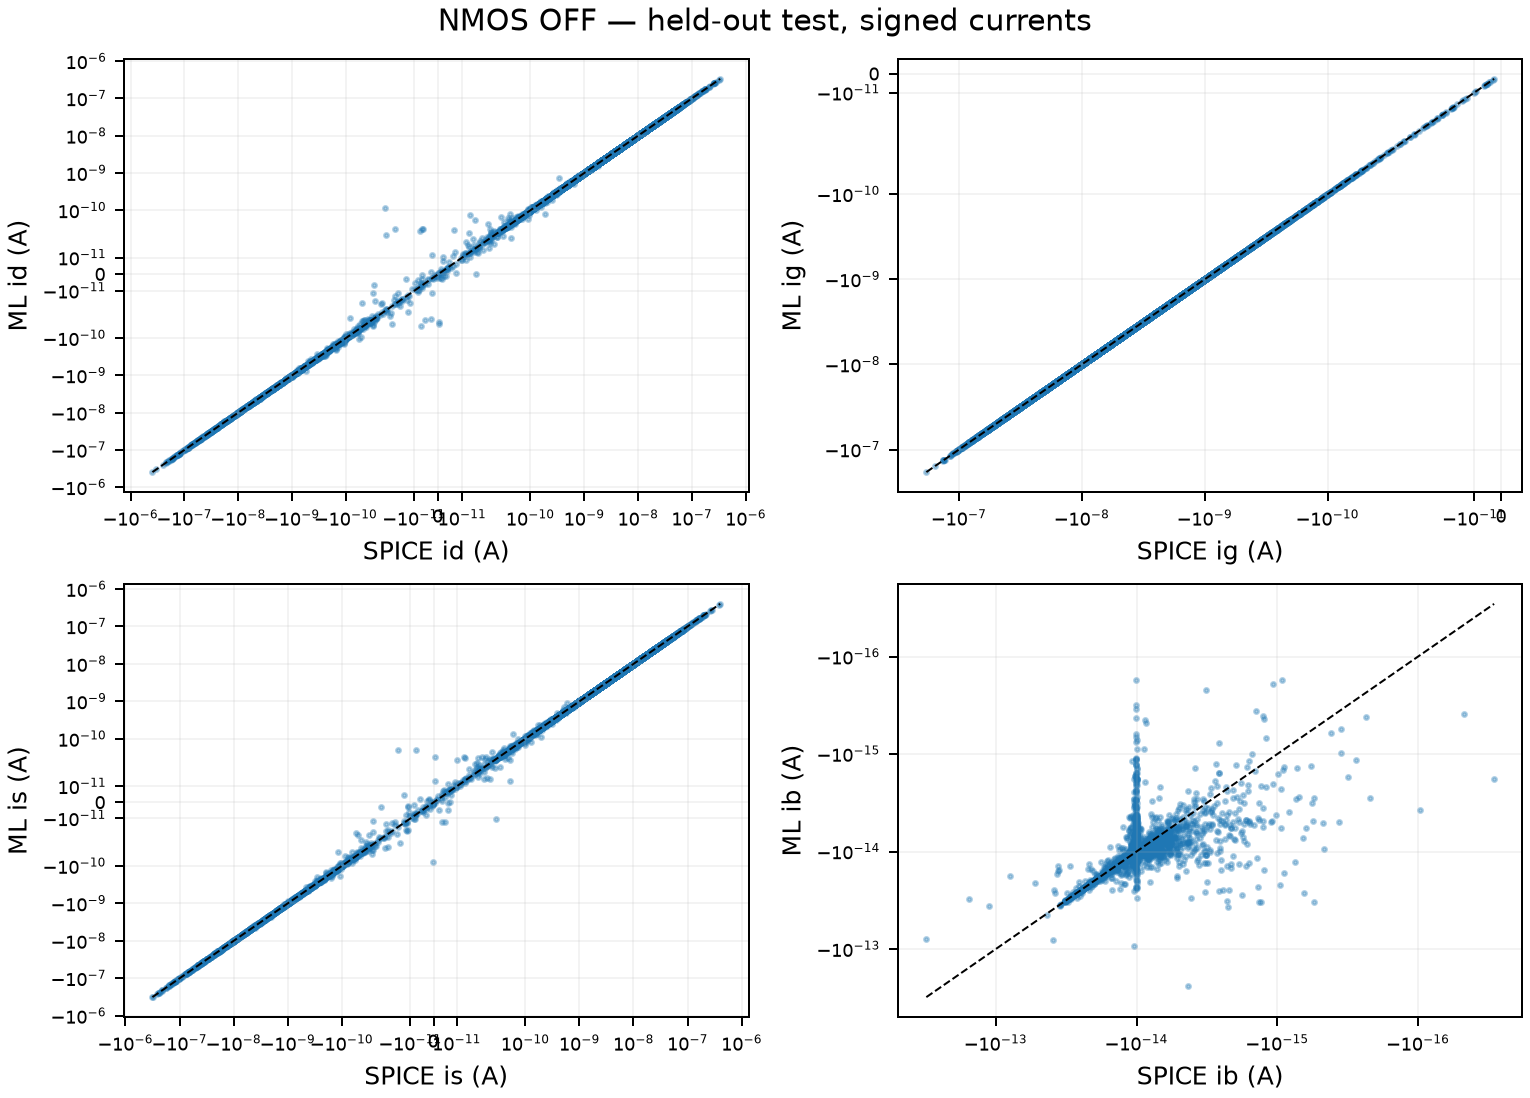
\includegraphics[width=\linewidth]{figures/nmos_off_parity.png}\caption{NMOS OFF}\end{subfigure}\par\medskip
\begin{subfigure}[t]{0.49\linewidth}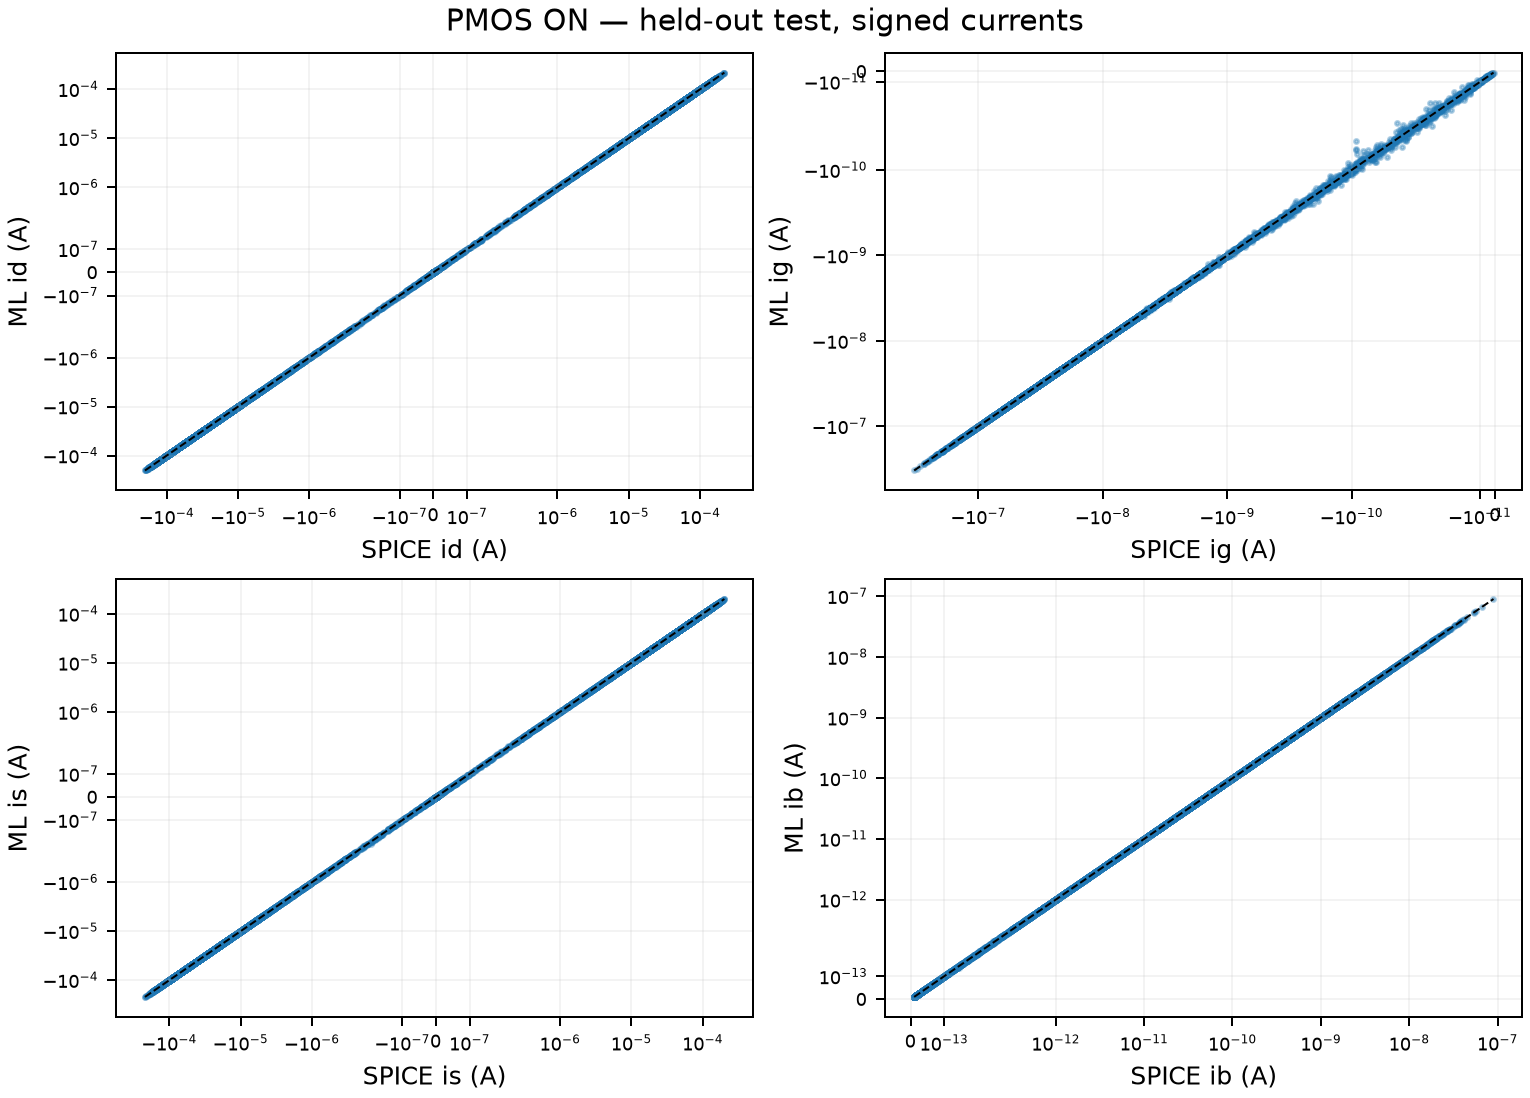
\includegraphics[width=\linewidth]{figures/pmos_on_parity.png}\caption{PMOS ON}\end{subfigure}
\begin{subfigure}[t]{0.49\linewidth}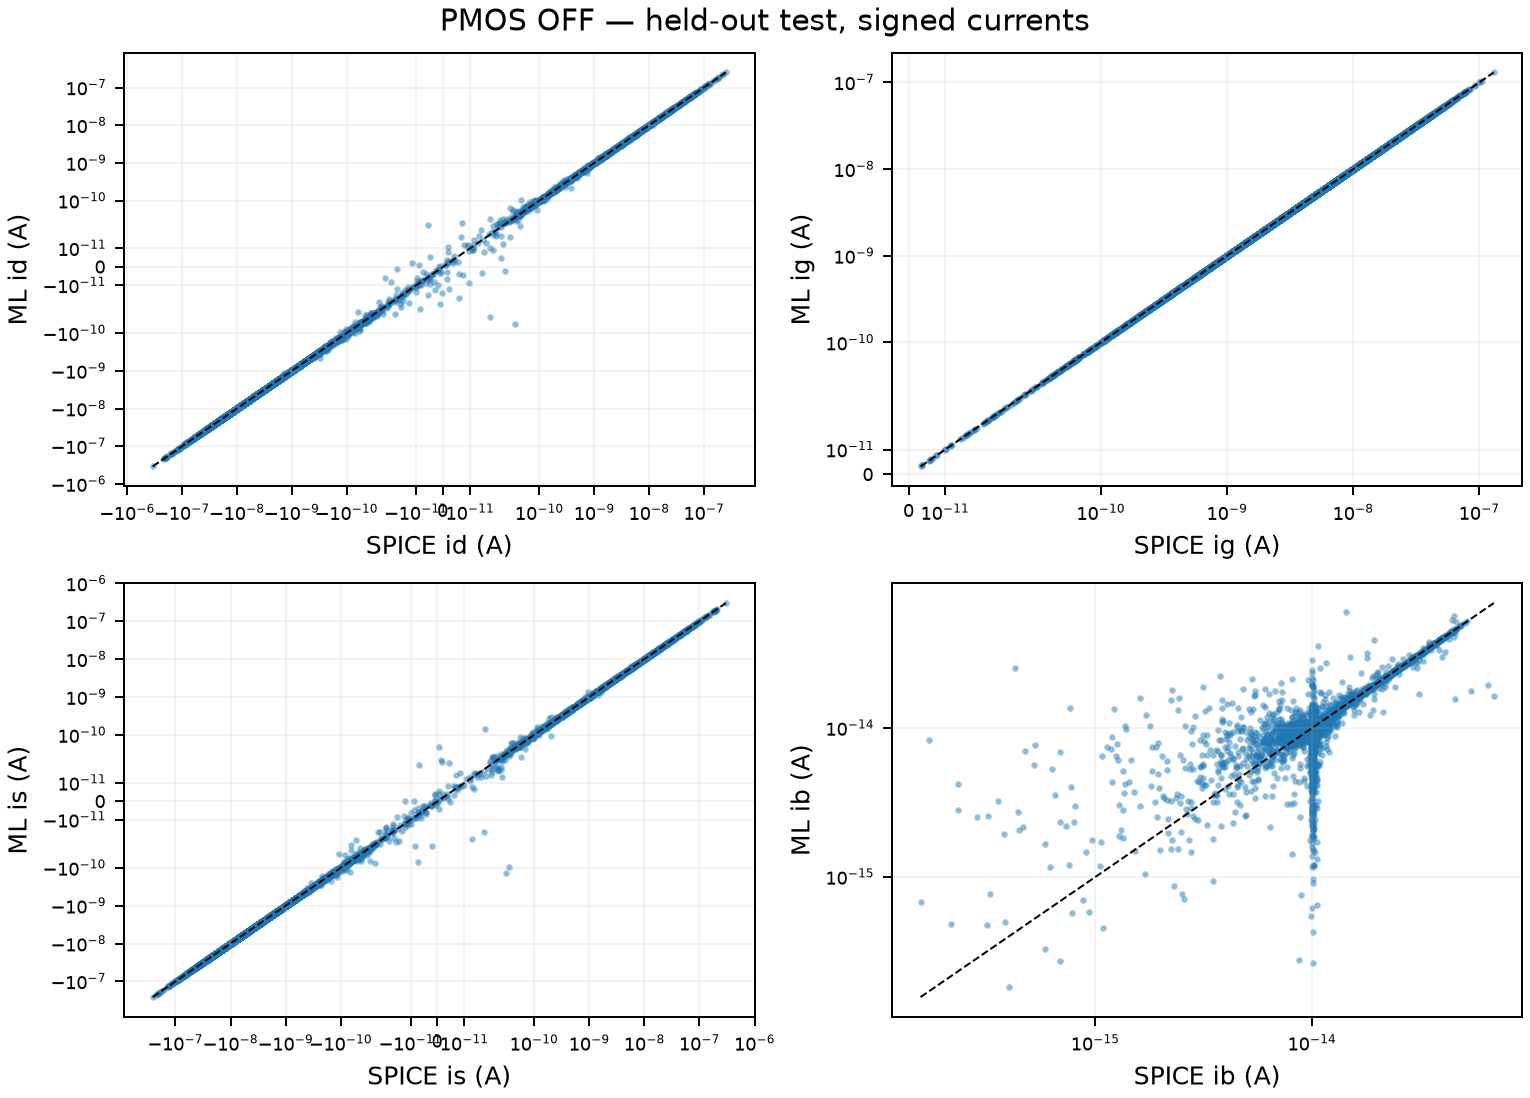
\includegraphics[width=\linewidth]{figures/pmos_off_parity.png}\caption{PMOS OFF}\end{subfigure}
\caption{Predicted against SPICE terminal currents on the 15,000 test rows of each case (symmetric-log axes; dashed line is equality).}
\label{fig:parity4}
\end{figure}
